\subsection{}
Understanding the logic of what a consumer goes through.
\par
If the price of good 1 goes down, there are two effects.
\begin{enumerate}
    \item Substitution Effect. If purchasing power stays the same, the money will stretch further, either more of good 1 or 2.
    If purchasing power changes with the price change, the consumer would want to purchase more of good 1 and less of good 2.
    \item Income Effect. Based on purchasing power change alone, how does the consumer feel. If the price of good 1 goes down, the consumer is richer.
\end{enumerate}
For a normal good, a price decrease, leads to a higher quantity demanded. But in a more complicated sense,
the consumer substitutes good 1 for good 2 (substitution effect) as well as purchasing more of good 1 due to being richer (income effect).\\
Substitution effect and income effect work in the same direction.
\begin{figure}[H]
    \centering
    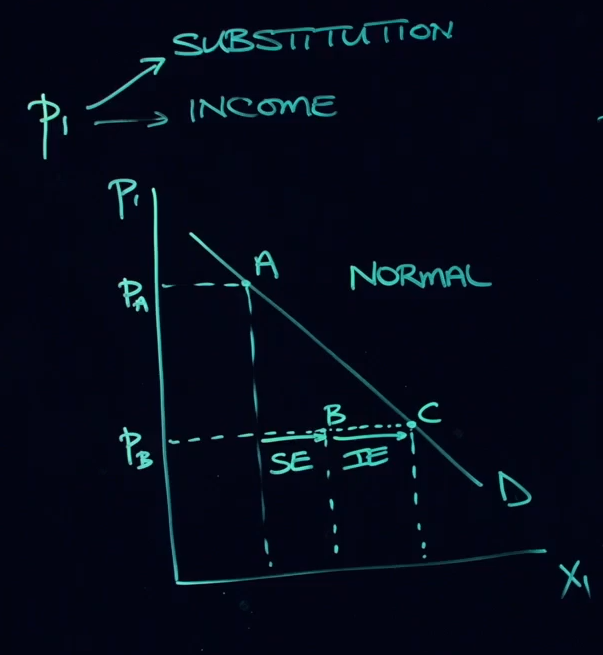
\includegraphics[width=0.5\textwidth]{Chapter6/NormalGood.png}
    \caption{Normal Good}
    \label{fig:Normal_Good}
\end{figure}\par
For an inferior good, a price decrease leads to the substitution effect and income effect working in opposite directions.
The consumer feels richer and doesn't want to buy the inferior good.
\begin{figure}[H]
    \centering
    
\includegraphics[width=0.5\textwidth]{Chapter6/InferiorGood.png}
    \caption{Inferior Good}
    \label{fig:Inferior_Good}
\end{figure}\par
There is a rare circumstance for an inferior good to be purchased even less after a price decrease.
The income effect outweighs the substitution effect. This is called a Giffen good. Giffen goods must be inferior. The circumstance
requires spending a large amount of income on the good, where the price change sends the consumer after better goods.
\begin{figure}[H]
    \centering
    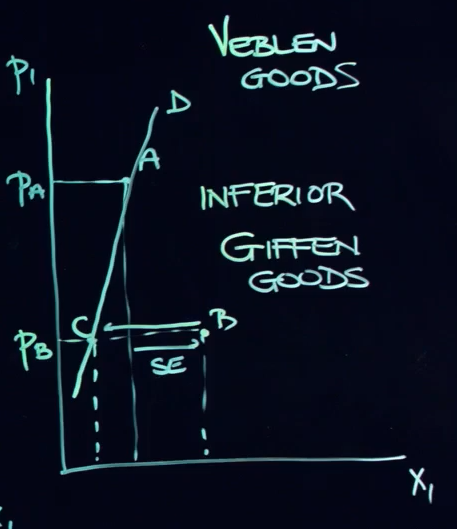
\includegraphics[width=0.5\textwidth]{Chapter6/GiffenGood.png}
    \caption{Giffen Good}
    \label{fig:Giffen_Good}
\end{figure}\par
Another scenario where this could happen is with Veblen goods. These are goods that are purchased for their status or the 
price contains something about the quality of the good.\\
The substitution effect is the change in quantity demanded that results from a change in 
relative prices while 
real income is/are 
constant
. The income effect is the change in quantity demanded that results from a change in 
real income while 
relative prices
is/are 
constant
.